\section{Related Work} \label{related work}

\subsection{Frequency deviation and modulation rate for warble tones}
\label{WarbleTones}



A study by W. Staab and W. Rintelmann \cite{warbleToneStatus} comparing the warble tone implementation of 6 different audiometer manufacturers found a large variety of frequency deviations and modulation rates across the manufacturers. Frequency deviation varied from $\pm$ 0.2$\%$ to $\pm$ 5$\%$, and the implemented modulation rate went from 2 Hz to 10 Hz. Another study by W. Staab \cite{warbleTonesComparison} comparing different warble-tone combinations on normal hearing (NH) adults found that frequency deviation up to $\pm$ 10$\%$ and modulation rates up to 32 Hz show little or no noticeable difference in results when compared to pure tones. Other studies suggest a range of different combinations, \cite{warbleEquation} use a frequency deviation of  $\pm$ 4.3$\%$ and a modulation rate of 4 Hz, \cite{warbleTesting} use a frequency deviation of $\pm$ 5$\%$  and a modulation rate of 5 Hz and \cite{warbleReliabilty} use a frequency deviation of $\pm$ 4$\%$ and modulation rate of 5 Hz. \newline

Considering the target group, warble tones must be implemented in the play audiometer, along with pure tones. Based on other studies, the warble tone should have a frequency deviation around  $\pm$ 4-5$\%$ but no higher than 10\% and a modulation rate around 4-5 Hz, but no higher than 32 Hz. However, the frequency deviation and modulation must also be changeable for the play audiometer to have the ability to match the warble tone of any audiometer. 

\subsection{Gamification of CPA} \label{gamification of CPA}

At CHBC, the analog version of CPA is still used to estimate hearing thresholds \cite{CFBH,loneConversation}. However, studies using tablet or computer-based games to automate and gamify CPA show promising results \cite{ipadAudiometry, self-administeredHL}. \newline

\begin{figure}[h]
    \centering
    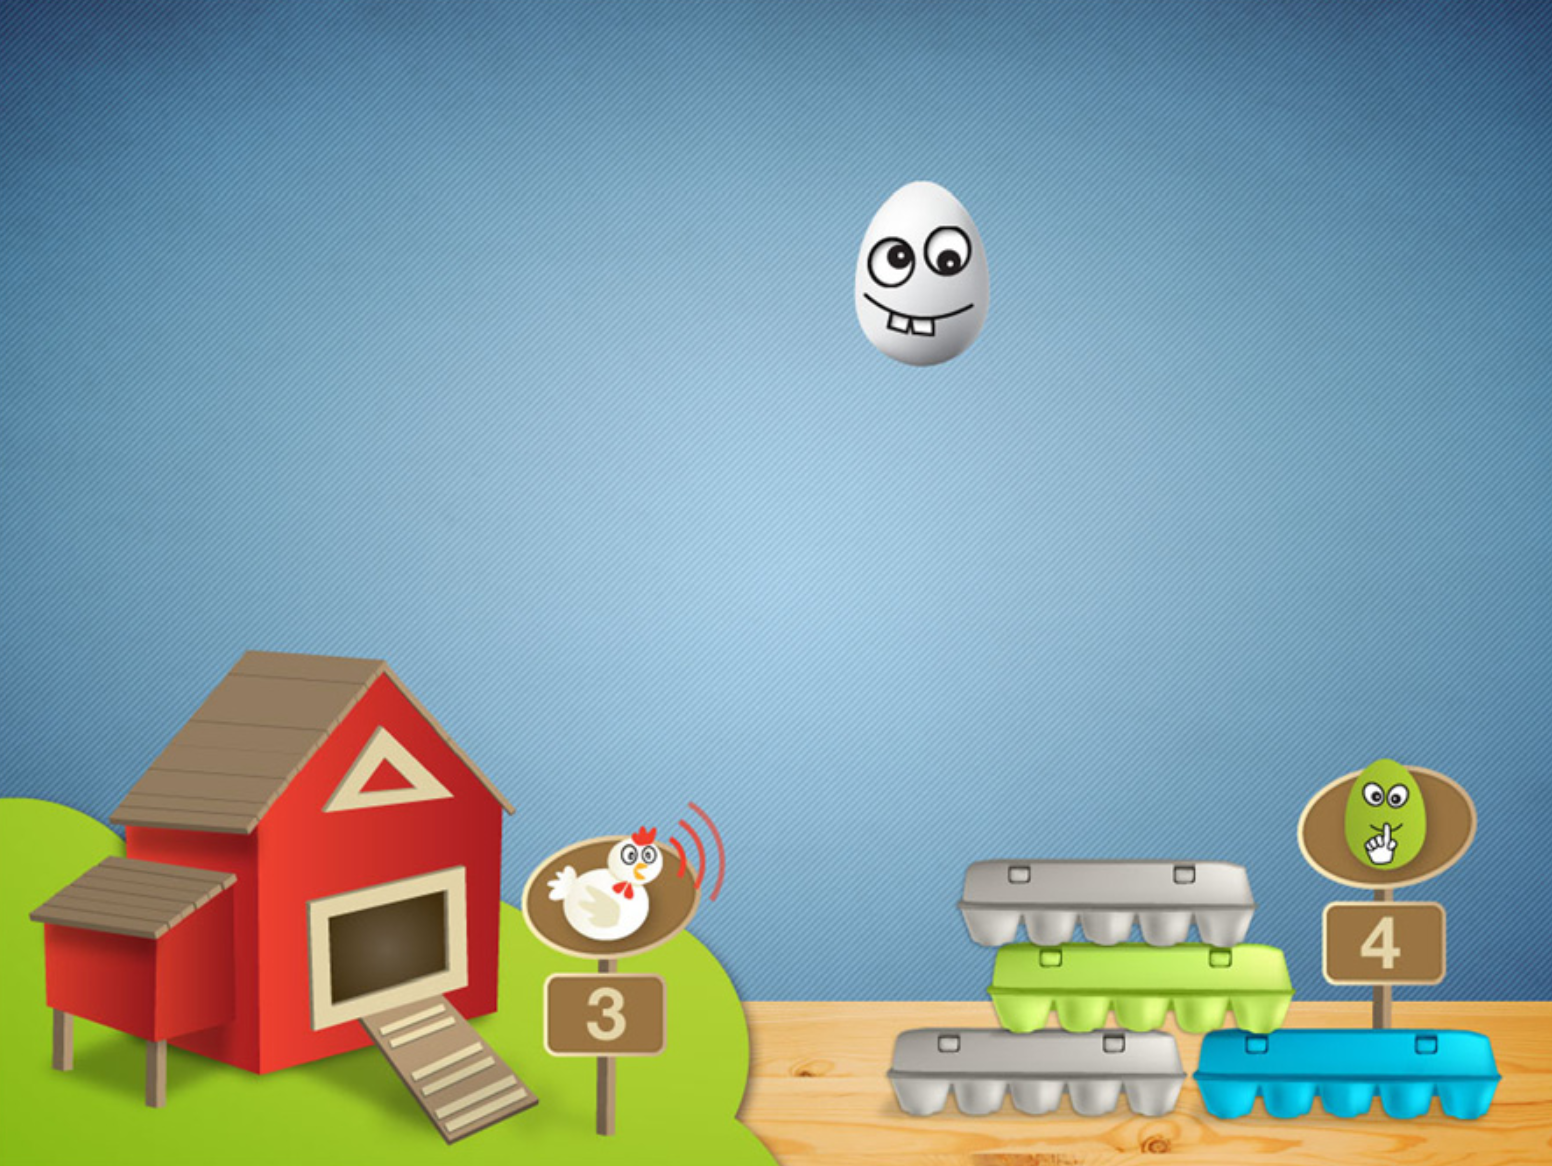
\includegraphics[width = 0.46\textwidth]{SMC2022_template_Latex/images/IpadAudiometry.png}
    \caption{Tablet audiometer gameplay screenshot \cite{ipadAudiometry}}
    \label{fig:ipadAudiometry}
\end{figure}

In a study by J. Yeung et al., a tablet-based play audiometer was implemented and evaluated to examine whether such a device can address the shortcomings (i.e., low patient cooperation) of the existing audiometry \cite{ipadAudiometry}. In the game, the child is presented with a series of objects (e.g., eggs) and is asked to categorize an object as 'silent' or 'sound-producing' by dragging the object into a container (see figure \ref{fig:ipadAudiometry}). The objects play warble tones at different frequencies. During the game, the intensity of the tones decreases until the child can no longer sort the objects correctly \cite{ipadAudiometry}. The study found that a tablet-based game is viable for testing children down to three years old. Furthermore, the study also demonstrated that there is no significant difference between the hearing threshold obtained by the device and thresholds obtained by standard play audiometry \cite{ipadAudiometry}. \newline 

The promising results from the tablet play audiometer show that it is possible to implement a computer-based game with the ability to collect the same results as traditional CPA.

\subsection{Azure Kinect for body tracking} \label{kinect}

Kinect is a popular tool used for rehabilitation and diagnostics because of the efficient skeleton tracking \cite{parkinsonKinect, balanceKinect, autismClassroom, tremorsKinect}. For children, studies show promising results when using Kinect in gamification applications \cite{autismGame, gamificationChildren}. 

\begin{figure}[h]
    \centering
    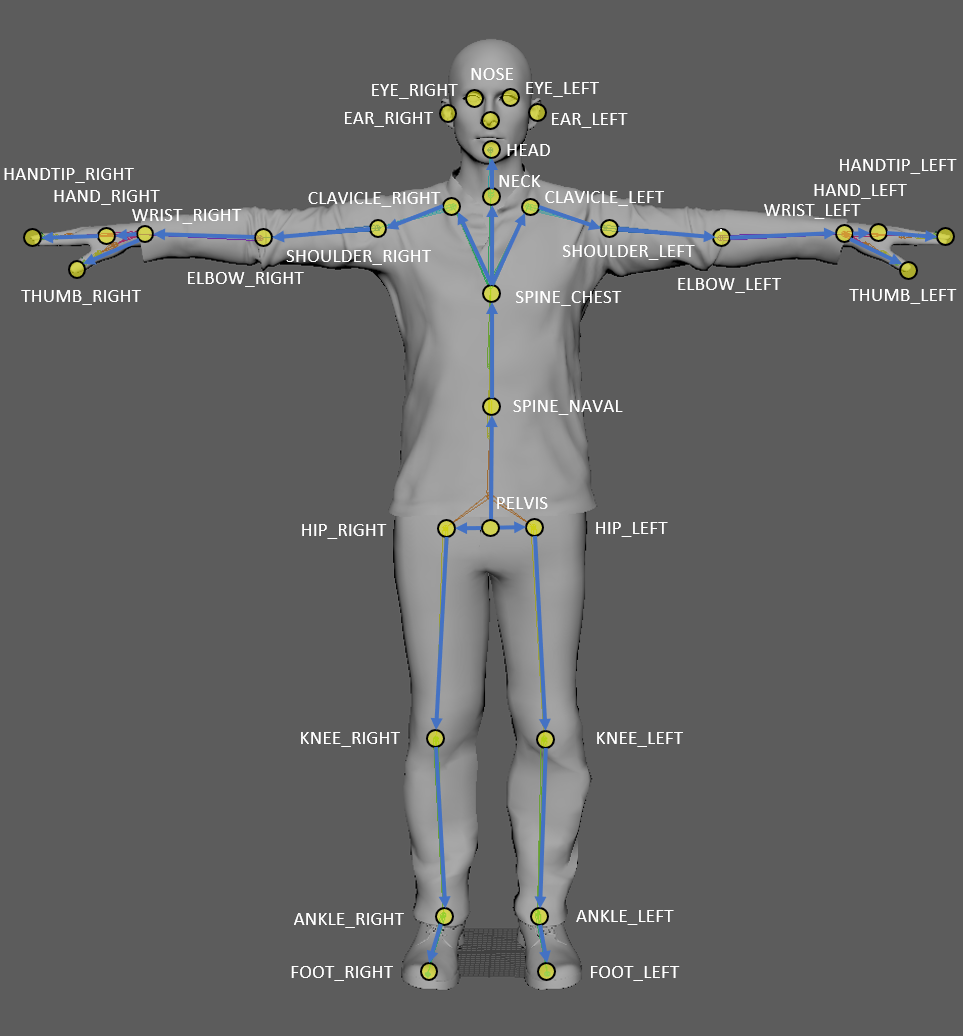
\includegraphics[width = 0.4\textwidth]{SMC2022_template_Latex/images/joint-hierarchy.png}
    \caption{The 32 tracked body joints by the Azure Kinect. All the joints are measured with position, and orientation/rotation \cite{kinectImage}.}
    \label{fig:skeletonTracked}
\end{figure}

Since 2010 three different versions of the Kinect have been released. The first version was initially designed as a game controller for the Xbox, and using an integrated RGB, and infrared camera allowed tracking users in 3D space \cite{kinectVS}. The third version of the Kinect (called Azure Kinect) has since been released in 2019 and enables skeleton tracking of 32 joints (see figure \ref{fig:skeletonTracked}) \cite{kinectVS}. A study by J. A. Albert et al., comparing the three released versions, has found that the skeleton and body tracking has been improved significantly from the first to the third version \cite{kinectVS}. \newline

The promising results from other studies and the significant body tracking development make the Azure Kinect a preferable tool for tracking the child's reaction and controlling the game. Additionally, the Azure Kinect is not body worn and hence more maneuverable and wireless, allowing the child to move more freely, creating a more immersive experience. 